\section{COMPARISON OF UU AND CU TEST RESULTS UU和CU试验结果的比较}

\begin{paracol}{2}
    
    \autoref{table:2} presents test data on nine soils from various locations in the world. Most of the soils are normally consolidated or slightly overconsolidated, $\overline{\sigma}_{vm}/\overline{\sigma}_{v0}$ equal to less than 3, lean to plastic clays with sensitivities below ten. Specimen depths varied from 0 to 35 m below ground surface. The strength values in Columns 4 and 5 are the averages from unconfined (U tests) and UU triaxial compression tests except for Case C as noted. The results of vane tests were not included in \autoref{table:2} since the interpretation of vane data is open to question.\footnote{
        The ratio of $S_u$ (UU) to vane strength averaged 0.85 (0.45 to 2.0) for Cases B, C, D, F, H, and I in \autoref{table:2}. \cntableref{table:2}中的情况B,C,D,F,H和I的$S_u$(UU)与叶片强度的比率平均为0.85(0.45至2.0)。
    }

    \switchcolumn

    \cntableref{table:2}列出了来自世界各地的9种土体的试验数据。 大多数土体通常是固结的或略有过固结的,$\overline{\sigma}_{vm}/\overline{\sigma}_{v0}$等于3以下,通常为敏感度低于10的塑料黏土。 标本深度在地面以下0到35 m之间变化。 第4列和第5列中的强度值是无限制(U试验)和UU三轴压缩试验的平均值,但情况C除外。 叶片试验的结果未包含在\cntableref{table:2}中,因为叶片的数据值得商榷。

    \switchcolumn*

    As Column 6 of \autoref{table:2} shows, the undrained strength as obtained from UU tests varies from 40 to 97 percent of the strength as obtained from CIU tests with $\overline{\sigma}_c=\overline{\sigma}_{v0}$, with an average value of 66 percent. In general, this ratio decreased with increasing depth of specimen.

    \switchcolumn

    如\cntableref{table:2}的第6列所示,UU试验获得的不排水强度$\overline{\sigma}_c=\overline{\sigma}_{v0}$时CIU试验获得的不排水强度的40$\%$至97$\%$,平均值为66$\%$。 通常,该比率随样品深度的增加而降低。

    \switchcolumn*

    A more detailed comparison of the results of $\overline{UU}$ and $\overline{CIU}$ tests on the Lagunillas clay, Case B of \autoref{table:2}, and the Kawasaki clays, Case C of \autoref{table:2}, is given in \autoref{figure:5} to \autoref{figure:10}. The tests on these normally consolidated clays were run on trimmed specimens 10 $\rm{cm^2}$ in area by 8 cm high using either the Norwegian Geotechnical Inst. (NGI) equipment \citep{Andresen1960695} or English equipment \citep{Bishop1962}. The NGI null device was used for the $\overline{CIU}$ tests; filter strips were placed on the test specimens, and backpressures of 1 to 3 $\rm{kg/cm^2}$ were employed. The rate of strain was about 1 percent/hr. A filter strip correction of 0.10 $\rm{kg/cm^2}$ was subtracted from measured values of ($\sigma_1-\sigma_3$) for axial strains exceeding 2 percent. The UU tests employed a fine porous base stone and Dynisco pressure transducer \citep{Whitman1961407}, no filter strips, a cell pressure of several $\rm{kg/cm^2}$, and a time to failure generally exceeding one day. All triaxial specimens were encased with two prophylactics with silicone grease; measured values of the B parameter before shear always exceeded 0.95 within 2 min. 

    \switchcolumn

    在\cntableref{table:2}的情况B的Lagunillas黏土和\cntableref{table:2}的情况C的Kawasaki黏土的$\overline{UU}$和$\overline{CIU}$试验结果的更详细比较在\cnfigureref{figure:5}至\cnfigureref{figure:10}。这些正常固结的黏土的试验是使用挪威岩土工程学院在面积10$\rm{cm^2}$高8cm的修整试样上进行的。 使用Norwegian Geotechnical Inst(NGI)设备\citep{Andresen1960695}或English设备\citep{Bishop1962}。NGI空设备用于$\overline{CIU}$试验; 将滤纸条放在试样上,并使用1至3$\rm{kg/cm^2}$的背压。 应变率约为1$\%$/小时。 如果轴向应变超过2$\%$,则从($\sigma_1-\sigma_3$)的测量值中减去0.10$\rm{kg/cm^2}$的滤带校正量。  UU试验使用了细的多孔基石和Dynisco压力传感器\citep{Whitman1961407},没有过滤带,电池压力为几$\rm{kg/cm^2}$,并且失效时间通常超过一天。 所有三轴试样均用硅脂润滑脂包裹了两种预防措施,剪切前B参数的测量值在2分钟内始终超过0.95。

    \begin{figure*}[!htbp]
    \centering
    \begin{minipage}[t]{0.48\textwidth}
        \centering
        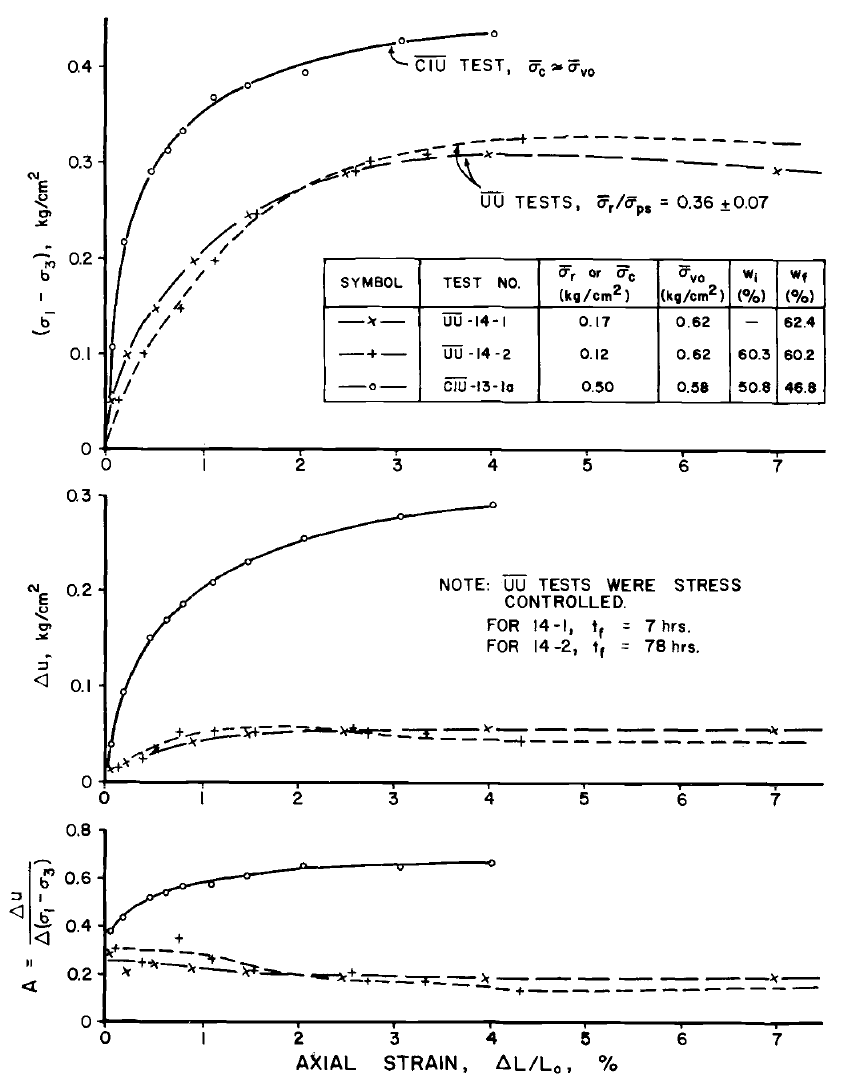
\includegraphics[width=0.9\textwidth]{figures/figure-5.png}
        \caption{Stress-Strain Data from Triaxial Tests on Lagunilas Clay.}
        \vspace{-5pt}
        \addtocounter{figure}{-1}
        \renewcommand{\figurename}{图}
        \caption{Lagunilas黏土的三轴试验的应力应变数据。}
        \label{figure:5}
        \renewcommand{\figurename}{Figure}
    \end{minipage}
    \begin{minipage}[t]{0.48\textwidth}
        \centering
        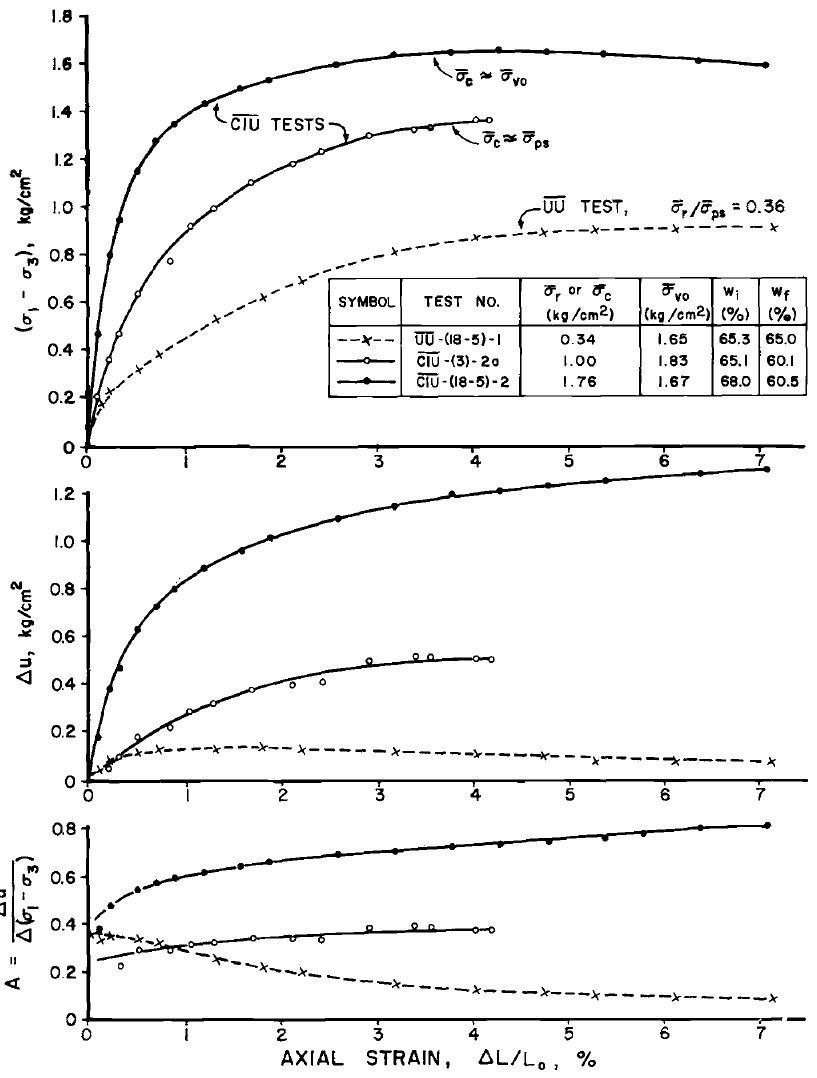
\includegraphics[width=0.9\textwidth]{figures/figure-6.png}
        \caption{Stress-Strain Data from Triaxial Tests on Kawasaki Clay I}
        \vspace{-5pt}
        \addtocounter{figure}{-1}
        \renewcommand{\figurename}{图}
        \caption{川崎黏土I的三轴试验的应力应变数据。}
        \label{figure:6}
        \renewcommand{\figurename}{Figure}
    \end{minipage}
\end{figure*}

    \begin{figure*}[!htbp]
    \centering
    \begin{minipage}[t]{0.48\textwidth}
        \centering
        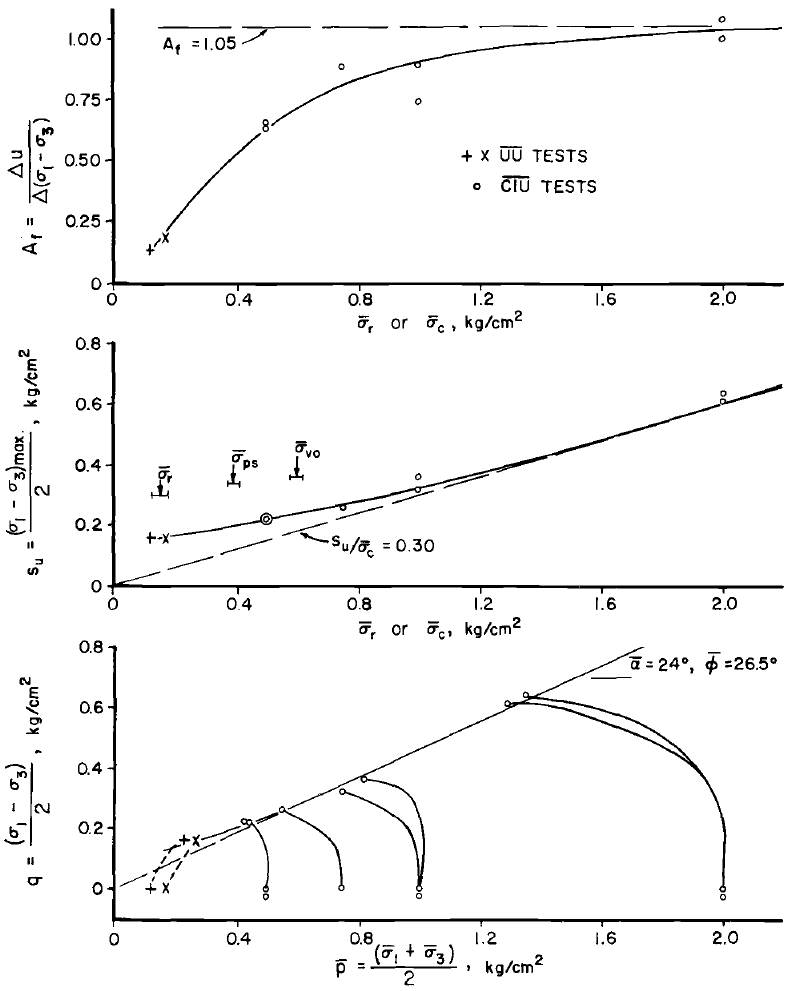
\includegraphics[width=0.9\textwidth]{figures/figure-7.png}
        \caption{Strength Data from Triaxial Tests on Lagunilas Clay.}
        \vspace{-5pt}
        \addtocounter{figure}{-1}
        \renewcommand{\figurename}{图}
        \caption{Lagunilas黏土的三轴试验的强度数据。}
        \label{figure:7}
        \renewcommand{\figurename}{Figure}
    \end{minipage}
    \begin{minipage}[t]{0.48\textwidth}
        \centering
        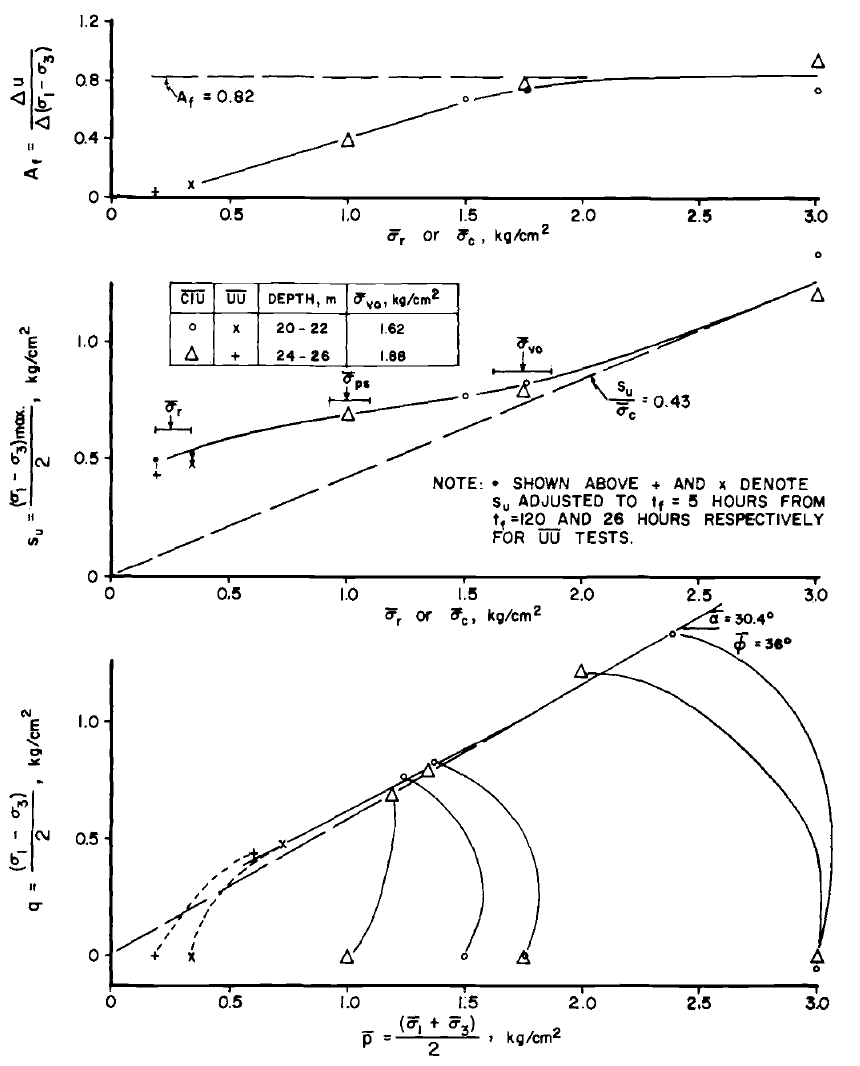
\includegraphics[width=0.9\textwidth]{figures/figure-8.png}
        \caption{Strength Data from Triaxial Tests on Kawasaki Clay I}
        \vspace{-5pt}
        \addtocounter{figure}{-1}
        \renewcommand{\figurename}{图}
        \caption{川崎黏土I的三轴试验的强度数据。}
        \label{figure:8}
        \renewcommand{\figurename}{Figure}
    \end{minipage}
\end{figure*}
    \begin{figure*}[!htbp]
    \centering
    \begin{minipage}[t]{0.48\textwidth}
        \centering
        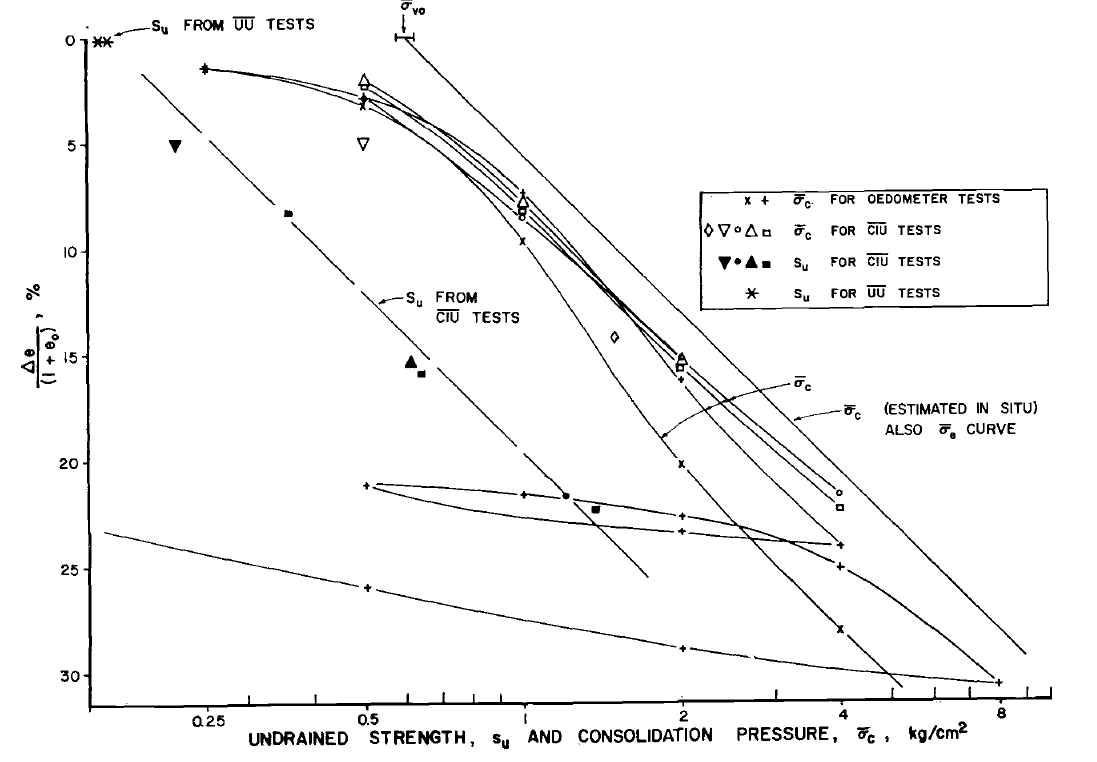
\includegraphics[width=0.9\textwidth]{figures/figure-9.png}
        \caption{Strength and Consolidation Pressure Versus Volumetric Strain on Lagunilas Clay.}
        \vspace{-5pt}
        \addtocounter{figure}{-1}
        \renewcommand{\figurename}{图}
        \caption{Lagunilas的黏土强度和固结压力与体积应变。}
        \label{figure:9}
        \renewcommand{\figurename}{Figure}
    \end{minipage}
    \begin{minipage}[t]{0.48\textwidth}
        \centering
        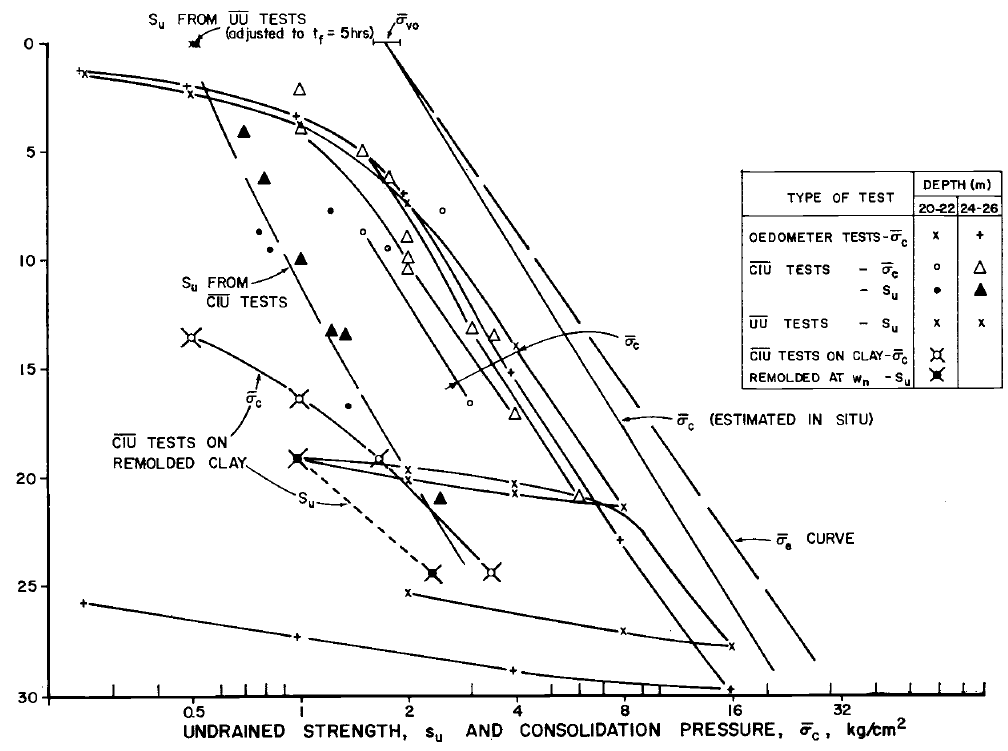
\includegraphics[width=0.9\textwidth]{figures/figure-10.png}
        \caption{Strength and Consolidation Pressure Versus Volumetric Strain on Kawasaki Clay I}
        \vspace{-5pt}
        \addtocounter{figure}{-1}
        \renewcommand{\figurename}{图}
        \caption{Lagunilas黏土I的强度和固结压力与体积应变。}
        \label{figure:10}
        \renewcommand{\figurename}{Figure}
    \end{minipage}
\end{figure*}
    \switchcolumn*

    The data in \autoref{figure:5} through \autoref{figure:10} show the following results:\footnote{
        Measured or estimated values of $\overline{\sigma}_r$, $\overline{\sigma}_{ps}$ and $\overline{\sigma}_{v0}$ are generally shown in the figures for reference. $\overline{\sigma}_r$,$\overline{\sigma}_{ps}$和$\overline{\sigma}_{v0}$的测量或估计值通常在图中显示,以供参考。
    }

    \switchcolumn
    
    从\cnfigureref{figure:5}至\cnfigureref{figure:10}中的数据可得出以下结果:

    \switchcolumn*

    \begin{enumerate}
        \item The undrained shear strength, $S_u$, from $\overline{UU}$ tests is only 70 to 85 percent of the value from $\overline{CIU}$ tests consolidated to the theoretical pressure corresponding to perfect sampling, that is, $\overline{\sigma}_c=\overline{\sigma}_{ps}$, (\autoref{figure:7} and \autoref{figure:8}). This difference in $S_u$ arises from the fact that the residual effective stress $\overline{\sigma}_r$, of the laboratory shear specimens is considerably less than the theoretical value $\overline{\sigma}_{ps}$. Identical strengths would have resulted if $\overline{\sigma}_r$, had equalled $\overline{\sigma}_{ps}$ since the preshear $\overline{\sigma}$ and void ratios would therefore have been equal for both tests.
        \item The slope of the stress-strain curve from $\overline{UU}$ tests is approximately one half of that from $\overline{CIU}$ tests with $\overline{\sigma}_c=\overline{\sigma}_{ps}$ (\autoref{figure:5} and \autoref{figure:6}).
        \item  There is good agreement among $\overline{UU}$ and $\overline{CIU}$ strength data if the $\overline{CIU}$ data are extrapolated backward so that the consolidation pressure equals $\overline{\sigma}_r$ (\autoref{figure:7} and \autoref{figure:8}) or the volumetric strain from the field condition is zero (\autoref{figure:9} and \autoref{figure:10}). This is to be expected since as the $\overline{\sigma}_c$ of $\overline{CIU}$ tests increased beyond $\overline{\sigma}_r$, there are corresponding increases in preshear $\overline{\sigma}$ and volumetric strain.
        \item As the consolidation pressure of $\overline{CIU}$ tests is increased from $\overline{\sigma}_{ps}$ to several times the in-situ vertical effective stress $\overline{\sigma}_{v0}$, $A_f$ shows a large increase and $S_u/\overline{\sigma}_c$ exhibits a marked decrease, whereas changes in the effective stress envelope are relatively minor (\autoref{figure:7}和\autoref{figure:8}).
        \item A relatively large volume decrease occurs when specimens are isotropically consolidated to pressures between $\overline{\sigma}_{ps}$ and $\overline{\sigma}_{v0}$ (\autoref{figure:9} and \autoref{figure:10}). Moreover, the oedometer test data\footnote{
        The fact that one of the oedonmter test eversus log$\overline{\sigma}_c$ curves in \autoref{figure:9} fell considerably below the curves for isotropic consolidation at high pressures is not considered typical. \cnfigureref{figure:9}中的oedonmter检验曲线log$\overline{\sigma}_c$曲线之一大大低于高压下的各向同性固结曲线,这一事实被认为是不典型的。
    } show that low values of $S_u/\overline{\sigma}_r$, indicating high disturbance, rather than an isotropic stress system \textit{per se}, are primarily responsible for the volume decrease.
    \end{enumerate}

    \switchcolumn

    \begin{enumerate}
        \item $\overline{UU}$试验的不排水剪切强度$S_u$仅为$\overline{CIU}$试验的固结至理论压力的70$\%$至85$\%$,即对应于完美采样的理论压力,即$\overline{\sigma}_c=\overline{\sigma}_{ps}$(\cnfigureref{figure:7}和\cnfigureref{figure:8})。$S_u$的差异是由于实验室剪切试样的残余有效应力$\overline{\sigma}_c$远小于理论值$\overline{\sigma}_{ps}$。 如果$\overline{\sigma}_c$等于$\overline{\sigma}_{ps}$,将产生相同的强度,因为预剪切力$\overline{\sigma}$和空隙率因此在两个试验中均相等。
        \item 若$\overline{\sigma}_c=\overline{\sigma}_{ps}$,$\overline{UU}$试验的应力-应变曲线的斜率约为$\overline{CIU}$试验的斜率的一半(\cnfigureref{figure:5}和\cnfigureref{figure:6})。
        \item 如果将$\overline{CIU}$数据向后外推,以使固结压力等于$\overline{\sigma}_r$(\cnfigureref{figure:7}和\cnfigureref{figure:8})或现场条件下的体积应变为零(\cnfigureref{figure:9}和\cnfigureref{figure:10}),则$\overline{UU}$和$\overline{CIU}$强度数据之间存在很好的一致性。这是可以预期的,因为随着$\overline{CIU}$试验的$\overline{\sigma}_c$增加到$\overline{\sigma}_r$以上,预剪力$\overline{\sigma}$和体积应变也会相应增加。
        \item 随着$\overline{CIU}$试验的固结压力从$\overline{\sigma}_{ps}$增加到原位垂直有效应力$\overline{\sigma}_{v0}$的几倍,$A_f$值显示出较大的增加,而$S_u/\overline{\sigma}_c$则显示出明显的降低,而有效应力包络线的变化相对较小(\cnfigureref{figure:7}和\cnfigureref{figure:8})。
        \item 当样品各向同性固结到$\overline{\sigma}_{ps}$和$\overline{\sigma}_{v0}$之间的压力时,体积会相对减小(\cnfigureref{figure:9}和\cnfigureref{figure:10})。此外,里程表试验数据表明,低值$S_u/\overline{\sigma}_r$表示高干扰,而不是各向同性应力系统本身,是体积减小的主要原因。
    \end{enumerate}

    \switchcolumn*
    
    These five trends are believed to be typical of tube specimens of normally consolidated, moderately sensitive, plastic clays which do not possess significant natural cementation.

    \switchcolumn
    
    这五个趋势被认为是通常固结,中等敏感性,不具有明显天然胶结作用的塑料黏土的试管样品的典型特征。

    \switchcolumn*

    \emph{In summary:} 

    \switchcolumn

    \emph{综上所述:}

    \switchcolumn*

    \begin{enumerate}
        \item Disturbance during tube sampling of normally consolidated clays may commonly decrease the effective stress of lab specimens by $80\pm{}20$ percent compared to perfect sampling.
        \item The resultant low values of $\overline{\sigma}_r$ cause the undrained strength $S_u$ from UU tests to be too low, whereas $S_u$ from CIU tests, which experience a significant volume decrease during consolidation, will most likely be too large.
        \item The ratio of $S_u$ from UU tests to that from CIU tests with $\overline{\sigma}_c=\overline{\sigma}_{ps}$ will typically be $75\pm{}25$ percent.
    \end{enumerate}

    \switchcolumn

    \begin{enumerate}
        \item 与完全采样相比,正常固结黏土的采样期间的干扰通常可能会使实验室标本的有效应力降低$80\%\pm{}20\%$。
        \item 所得的$\overline{\sigma}_r$值较低,导致UU试验的不排水强度$S_u$太低,而CIU试验的$S_u$则在固结过程中体积明显减小,很可能太大。
        \item $\overline{\sigma}_c=\overline{\sigma}_{ps}$的UU试验与CIU试验的$S_u$比率通常为$75\%\pm{}25\%$。
    \end{enumerate}

\end{paracol}